\begin{event}{6th Encuentro Colombiano de Combinatoria }{ECCO}{Barranquilla (Colombia), June 5 --- 16, 2018}{PS}{80}{1}{http://ecco2018.combinatoria.co/}

\textbf{Main goals.} ECCO (for \textit{Encuentro Colombiano de Combinatoria}) is a combinatorics research school organized every other year in Colombia. It gathered students from many countries (from both south-America and elsewhere) on advanced mathematics classes in an inclusive and welcoming environment. For the second time, it offered a \Sage class as well which goal is introduce \Sage to the students and help them develop their coding skills in relations to mathematics.

\textbf{ODK implication.} The \Sage class was given by Viviane Pons from ODK. Her travel costs were covered by ODK.

\textbf{Event summary.} Two afternoon sessions were organized (one for each week of the workshop). We had approximately 80 students on the first session and 40 on the second. Both sessions were organized in the computer room of the university so that all students would work whether they had material or not. Focus was given to introduction to \Sage in the context of combinatorics by offering many different tutorials and exercise worksheets for the students to choose from. We had created some specific worksheets in both English and Spanish directly related to the others courses of the conference so that the students could reproduce some of the results they had seen during classes and exercise sessions.

\textbf{Demographic.} We don't have access to the demographic information of the conference. Nevertheless we can say that most participants were students (from undergrad to PhD). Beside, this conference is in general very careful in creating a diverse and welcoming space.

\textbf{Results and impact.} This was the second time that we were at ECCO and we could see again that this was a great success. We had excellent feedbacks from both the students and the organizers. In 2016, the \Sage sessions were added late in the planning as extra sessions. In 2018, this is now an official \Sage course listed along the other mathematical classes of the conference. By being present twice in a row, we started a tradition of offering \Sage classes during this conference and this will be continued even after the end of ODK. For many students attending ECCO, the \Sage class is their first encounter with \Sage or even a mathematic software.

\begin{figure}[ht]
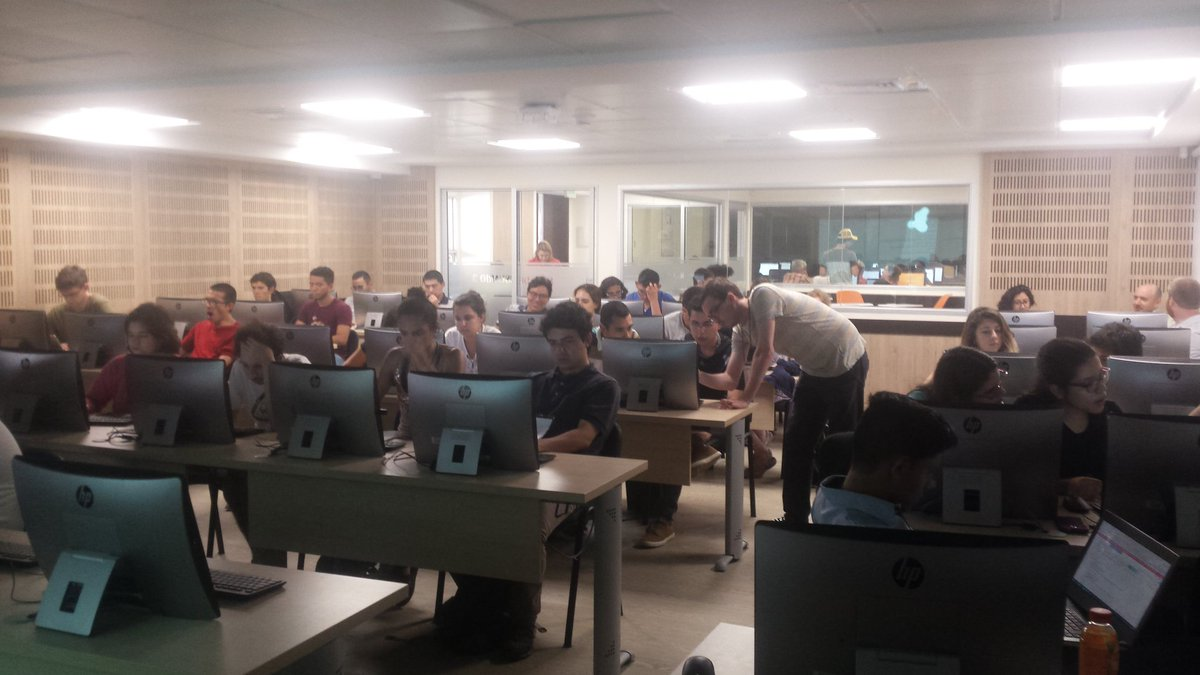
\includegraphics[scale=.2]{ECCO.jpg}
\caption*{Students working at ECCO}
\end{figure}



\end{event}